\documentclass[tikz,border=5pt]{standalone}
\usepackage[utf8]{inputenc}
\usepackage[T1]{fontenc}
\usepackage{lmodern,amsmath,amssymb}
\usepackage[american]{circuitikz}
\usepackage{pgfplots}
\pgfplotsset{compat=1.18}
\usetikzlibrary{circuits.logic.US,positioning,calc,arrows.meta,patterns,shapes.geometric}
\definecolor{Primary}{HTML}{1F77B4}
\begin{document}
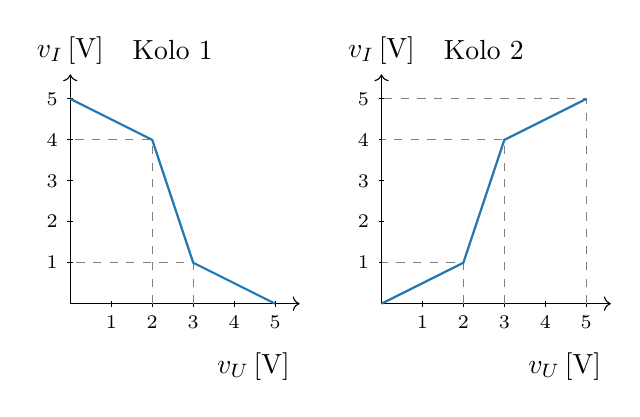
\begin{tikzpicture}[scale=.52]\begin{scope}[xshift=0.0cm]\draw[->] (0,0)--(5.6,0);\node[anchor=north east]at(5.6,-.95){$v_U\,[\mathrm V]$};\draw[->] (0,0)--(0,5.6) node[above]{$v_I\,[\mathrm V]$};\foreach \x in {1,...,5}{\draw (\x,.07)--(\x,-.07) node[below,font=\scriptsize]{\x};\draw (.07,\x)--(-.07,\x) node[left,font=\scriptsize]{\x};}\draw[dashed,gray] (2,0)|-(0,4);\draw[dashed,gray] (3,0)|-(0,1);\draw[Primary,thick] (0,5)--(2,4)--(3,1)--(5,0);\node at(2.5,6.2){Kolo 1};\end{scope}\begin{scope}[xshift=7.6cm]\draw[->] (0,0)--(5.6,0);\node[anchor=north east]at(5.6,-.95){$v_U\,[\mathrm V]$};\draw[->] (0,0)--(0,5.6) node[above]{$v_I\,[\mathrm V]$};\foreach \x in {1,...,5}{\draw (\x,.07)--(\x,-.07) node[below,font=\scriptsize]{\x};\draw (.07,\x)--(-.07,\x) node[left,font=\scriptsize]{\x};}\draw[dashed,gray] (2,0)|-(0,1);\draw[dashed,gray] (3,0)|-(0,4);\draw[dashed,gray] (5,0)|-(0,5);\draw[Primary,thick] (0,0)--(2,1)--(3,4)--(5,5);\node at(2.5,6.2){Kolo 2};\end{scope}\end{tikzpicture}
\end{document}
